\documentclass[french,a4paper,10pt]{article}
% pdflatex compte_rendu.tex -output-directory=out && mv out/compte_rendu.pdf ./

\usepackage[a4paper,hmargin=30mm,vmargin=30mm]{geometry}
\usepackage[T1]{fontenc} % font type
\usepackage[french]{babel} % language
\usepackage{lmodern} % font type
\usepackage[shortlabels]{enumitem}
\usepackage{hyperref}
\usepackage{graphicx}
\usepackage{sectsty}
%\setlength{\parindent}{0pt}



\title{Compte Rendu TP3\\Filtre inverse vidéo et floutages d'images}
\author{Ivan Lejeune}
\date{\today}


\begin{document}
    \maketitle

    % make table of contents
    \tableofcontents

    \newpage
    \section{Choix des images, histogramme et profil de ligne}\label{sec:1}

    \subsection{Choix de l'image}\label{subsec:1.1}

    On commence par choisir une image au format \emph{ppm}, dans notre cas, l'image \texttt{peppers.pgm}.
    On la transforme ensuite en \emph{pgm}.
    Cela donne alors :
    % insert original image and resized image
    \begin{figure}[!htb]
        \begin{minipage}{0.48\textwidth}
            \centering
            \fbox{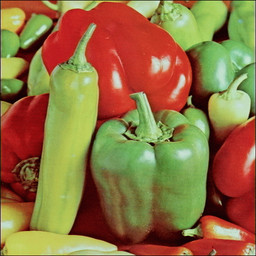
\includegraphics[width=.7\linewidth]{./out/orig-peppers}}
            \caption{Image originale}\label{Fig:orig-08}
        \end{minipage}\hfill
        \begin{minipage}{0.48\textwidth}
            \centering
            \fbox{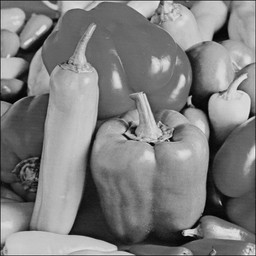
\includegraphics[width=.7\linewidth]{./out/peppers-grey}}
            \caption{Image en niveaux de gris}\label{Fig:resize-08}
        \end{minipage}
    \end{figure}

    \subsection{Histogramme}\label{subsec:1.2}

    On commence par calculer l'histogramme de l'image.
    Et ensuite le profil de ligne de l'image.
    On choisit ici la ligne 30.
    Cela donne :
    % insert histogram and line profile
    \begin{figure}[!htb]
        \begin{minipage}{0.48\textwidth}
            \centering
            \fbox{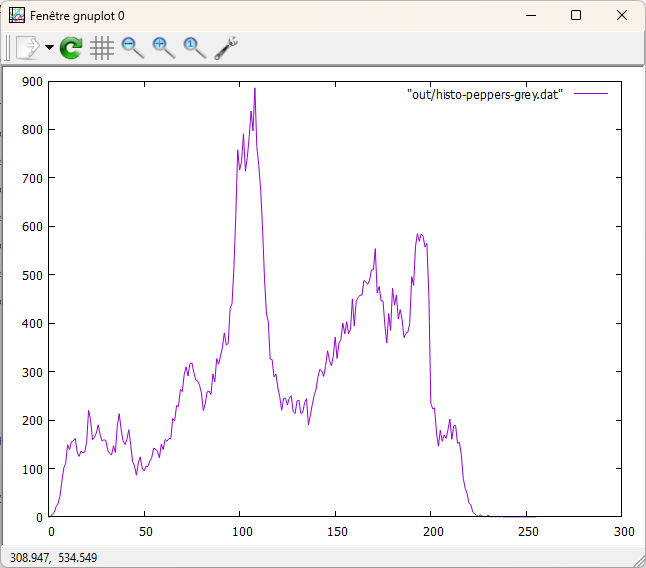
\includegraphics[width=.7\linewidth]{./out/histo-peppers-grey}}
            \caption{Histogramme de l'image en niveaux de gris}\label{Fig:histo-peppers-grey}
        \end{minipage}\hfill
        \begin{minipage}{0.48\textwidth}
            \centering
            \fbox{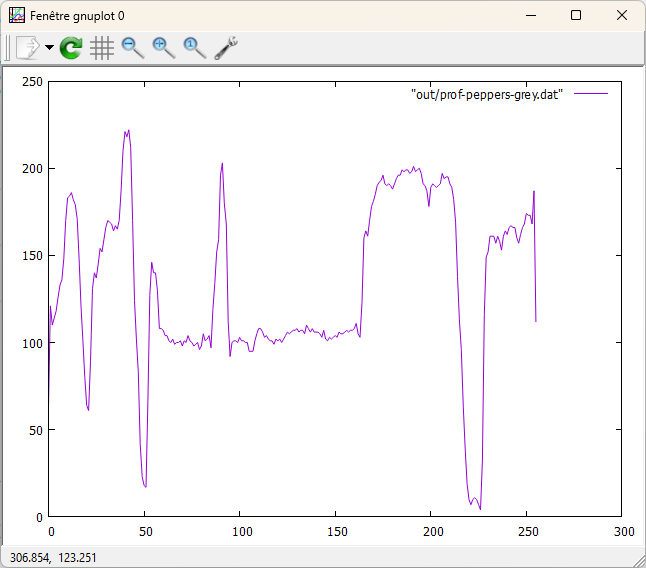
\includegraphics[width=.7\linewidth]{./out/prof-peppers-grey}}
            \caption{Profil de ligne de l'image en niveaux de gris}\label{Fig:prof-peppers-grey}
        \end{minipage}
    \end{figure}

    \newpage
    \section{Inverse vidéo}\label{sec:2}

    On commence par créer le programme \texttt{inverse.cpp}.
    L'essentiel du code est le suivant :
    % insert code as image
    \begin{figure}[!htb]
        \centering
        \fbox{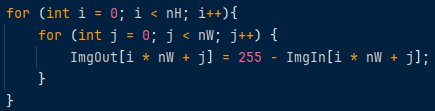
\includegraphics[width=.7\linewidth]{./out/code-inverse}}
        \caption{Code du programme \texttt{inverse.cpp}}\label{Fig:code-inverse}
    \end{figure}

    On peut alors appliquer le programme à l'image \texttt{peppers.pgm}.
    Cela donne :
    % insert image and modified image side by side
    \begin{figure}[!htb]
            \begin{minipage}{0.48\textwidth}
                \centering
                \fbox{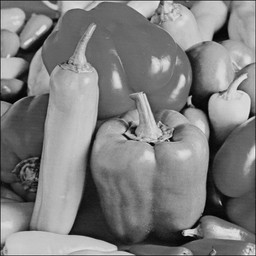
\includegraphics[width=.7\linewidth]{./out/peppers-grey}}
                \caption{Image originale}\label{Fig:peppers-grey}
            \end{minipage}\hfill
            \begin{minipage}{0.48\textwidth}
                \centering
                \fbox{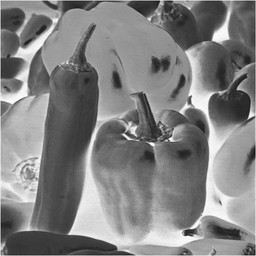
\includegraphics[width=.7\linewidth]{./out/peppers-grey-inverse}}
                \caption{Image inversée}\label{Fig:peppers-grey-inverse}
            \end{minipage}
        \end{figure}

    \subsection{Comparaison des profils de ligne}\label{subsec:2.1}

    On compare ensuite le profil de ligne de l'image originale et de l'image inversée.
    Cela donne :
    % insert line profile and modified line profile side by side
    \begin{figure}[!htb]
        \begin{minipage}{0.48\textwidth}
            \centering
            \fbox{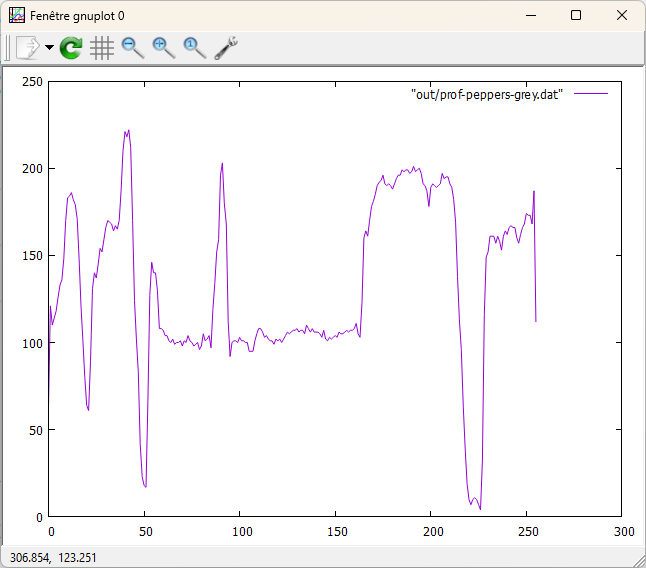
\includegraphics[width=.7\linewidth]{./out/prof-peppers-grey}}
            \caption{Profil de ligne de l'image originale}\label{Fig:prof-peppers-grey-1}
        \end{minipage}\hfill
        \begin{minipage}{0.48\textwidth}
            \centering
            \fbox{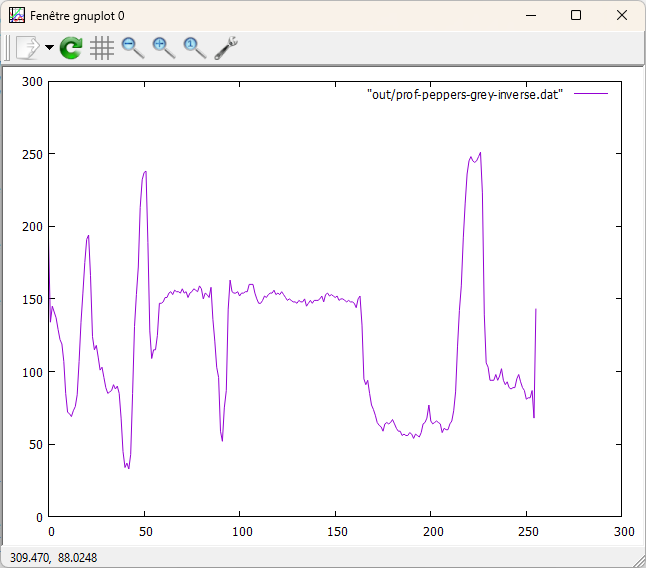
\includegraphics[width=.7\linewidth]{./out/prof-peppers-grey-inverse}}
            \caption{Profil de ligne de l'image inversée}\label{Fig:prof-peppers-grey-inverse}
        \end{minipage}
    \end{figure}

    On remarque que le profil de ligne de l'image inversée est l'opposé de celui de l'image originale.

    \newpage
    \section{Filtre flou 1}\label{sec:3}

    \subsection{Programme}\label{subsec:3.1}

    On commence par créer le programme \texttt{flou1.cpp}.
    L'essentiel du code est le suivant :
    % insert code as image
    \begin{figure}[!htb]
        \centering
        \fbox{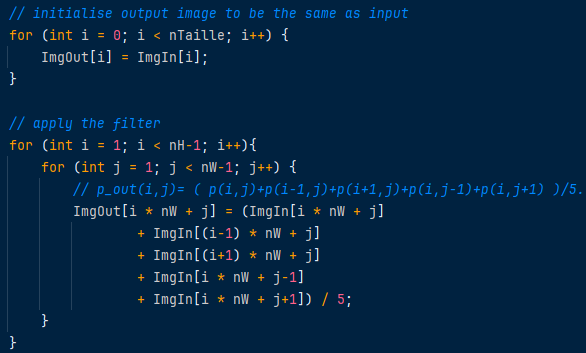
\includegraphics[width=.7\linewidth]{./out/code-filtre-flou1}}
        \caption{Code du programme \texttt{filtre\_flou1.cpp}}\label{Fig:code-filtre-flou1}
    \end{figure}

    On peut alors appliquer le programme à l'image \texttt{peppers.pgm}.
    Cela donne :
    % insert image and modified image side by side
    \begin{figure}[!htb]
        \begin{minipage}{0.48\textwidth}
            \centering
            \fbox{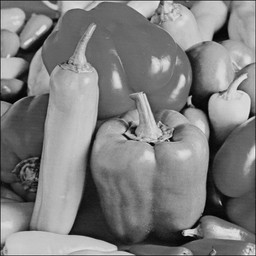
\includegraphics[width=.7\linewidth]{./out/peppers-grey}}
            \caption{Image originale}\label{Fig:peppers-grey-1}
        \end{minipage}\hfill
        \begin{minipage}{0.48\textwidth}
            \centering
            \fbox{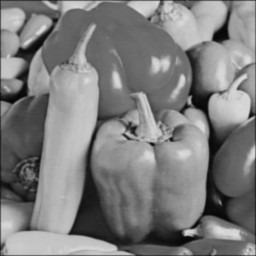
\includegraphics[width=.7\linewidth]{./out/peppers-grey-ff1}}
            \caption{Image floutée}\label{Fig:peppers-grey-ff1}
        \end{minipage}
    \end{figure}

    \newpage
    \subsection{Comparaison des profils de ligne}\label{subsec:3.2}

    On compare ensuite le profil de ligne de l'image originale et de l'image floutée.
    Cela donne :
    % insert line profile and modified line profile side by side
    \begin{figure}[!htb]
        \begin{minipage}{0.48\textwidth}
            \centering
            \fbox{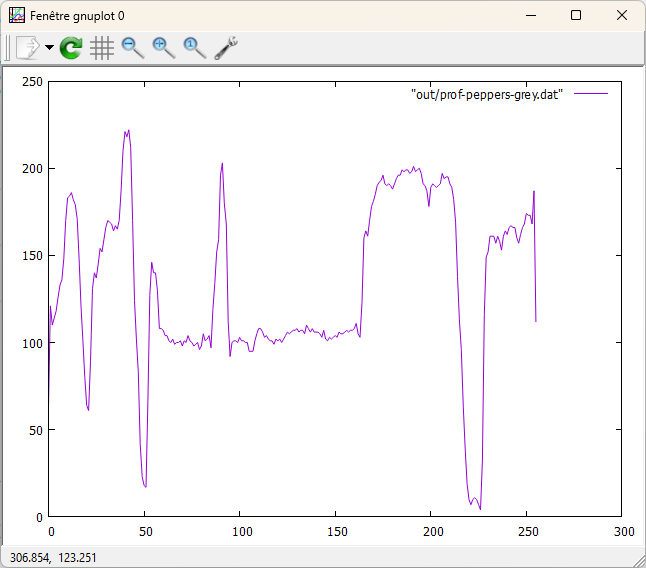
\includegraphics[width=.7\linewidth]{./out/prof-peppers-grey}}
            \caption{Profil de ligne de l'image originale}\label{Fig:prof-peppers-grey-2}
        \end{minipage}\hfill
        \begin{minipage}{0.48\textwidth}
            \centering
            \fbox{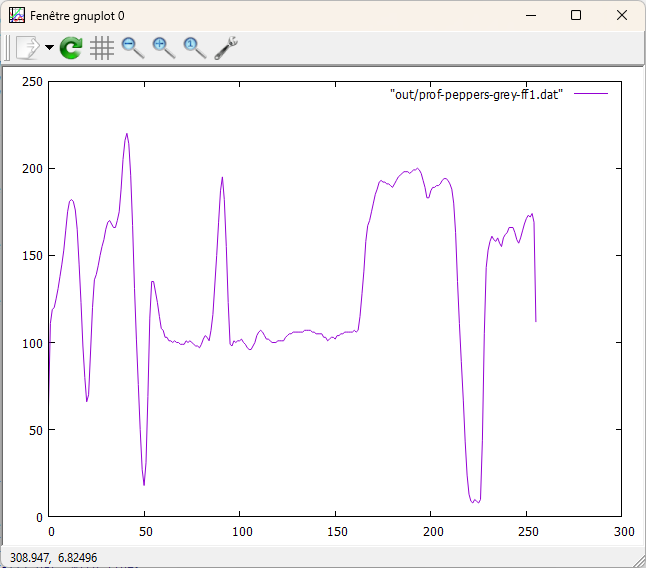
\includegraphics[width=.7\linewidth]{./out/prof-peppers-grey-ff1}}
            \caption{Profil de ligne de l'image floutée}\label{Fig:prof-peppers-grey-ff1}
        \end{minipage}
    \end{figure}

    On remarque que le profil de ligne de l'image floutée est plus lisse que celui de l'image originale.

    \newpage
    \section{Filtre flou 2}\label{sec:4}

    \subsection{Programme}\label{subsec:4.1}

    On commence par créer le programme \texttt{flou2.cpp}.
    L'essentiel du code est le suivant :
    % insert code as image
    \begin{figure}[!htb]
        \centering
        \fbox{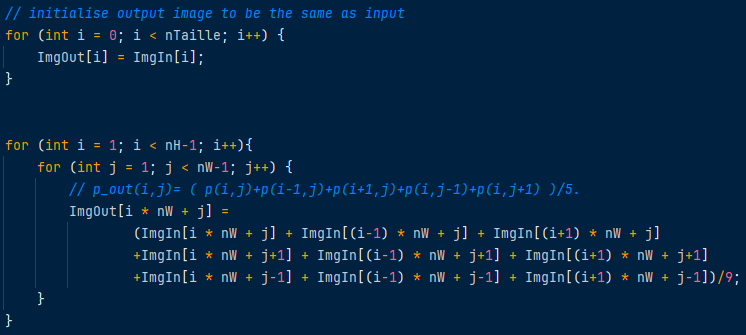
\includegraphics[width=.7\linewidth]{./out/code-filtre-flou2}}
        \caption{Code du programme \texttt{filtre\_flou2.cpp}}\label{Fig:code-filtre-flou2}
    \end{figure}

    On peut alors appliquer le programme à l'image \texttt{peppers.pgm}.
    Cela donne :
    % insert image and modified image side by side
    \begin{figure}[!htb]
        \begin{minipage}{0.48\textwidth}
            \centering
            \fbox{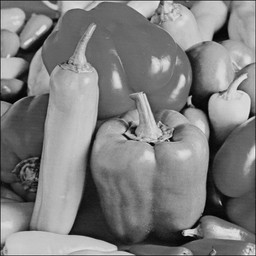
\includegraphics[width=.7\linewidth]{./out/peppers-grey}}
            \caption{Image originale}\label{Fig:peppers-grey-2}
        \end{minipage}\hfill
        \begin{minipage}{0.48\textwidth}
            \centering
            \fbox{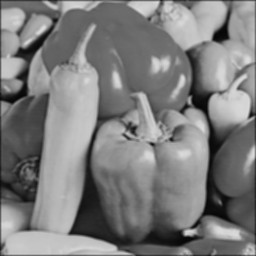
\includegraphics[width=.7\linewidth]{./out/peppers-grey-ff2}}
            \caption{Image floutée}\label{Fig:peppers-grey-ff2}
        \end{minipage}
    \end{figure}

    \newpage
    \subsection{Floutage répété}\label{subsec:4.2}

    On applique ensuite le programme \texttt{flou2.cpp} à l'image floutée plusieurs fois.
    Cela donne :
    % insert image and modified image side by side
    \begin{figure}[!htb]
        \begin{minipage}{0.48\textwidth}
            \centering
            \fbox{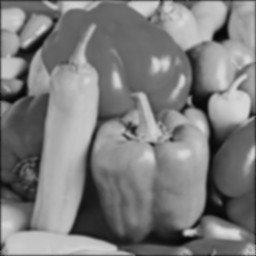
\includegraphics[width=.7\linewidth]{./out/peppers-grey-ff2-2}}
            \caption{Image floutée deux fois}\label{Fig:peppers-grey-ff2-2}
        \end{minipage}\hfill
        \begin{minipage}{0.48\textwidth}
            \centering
            \fbox{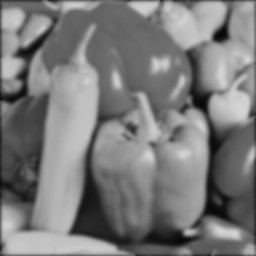
\includegraphics[width=.7\linewidth]{./out/peppers-grey-ff2-5}}
            \caption{Image floutée cinq fois}\label{Fig:peppers-grey-ff2-5}
        \end{minipage}
    \end{figure}

    \newpage
    \subsection{Comparaison des profils de ligne}\label{subsec:4.3}

    On compare ensuite le profil de ligne de l'image originale et de toutes les images floutées.
    Cela donne :
    % insert graph of line profiles
    \begin{figure}[!htb]
        \centering
        \fbox{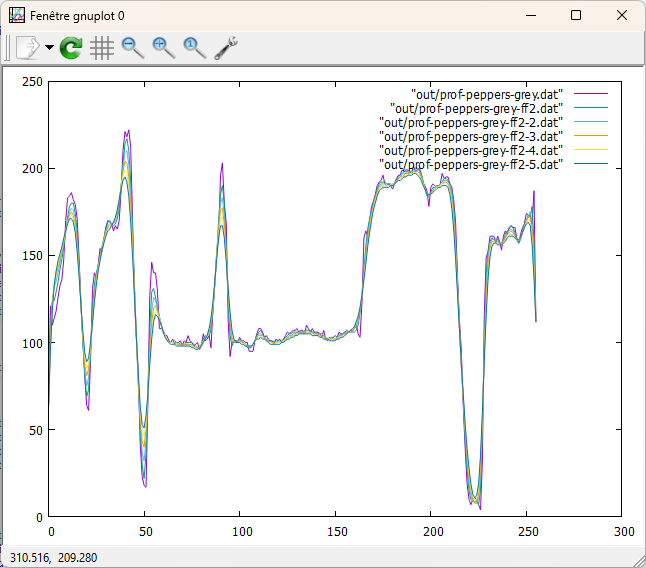
\includegraphics[width=.7\linewidth]{./out/prof-peppers-grey-ff2}}
        \caption{Profil de ligne de l'image floutée}\label{Fig:prof-peppers-grey-ff2}
    \end{figure}

    On peut clairement voir ici que plus on floute l'image, plus le profil de ligne devient lisse.

    \newpage
    \subsection{Comparaison des histogrammes}\label{subsec:4.4}

    On compare ensuite les histogrammes de l'image originale et de toutes les images floutées.
    Cela donne :
    % insert graph of histograms
    \begin{figure}[!htb]
        \centering
        \fbox{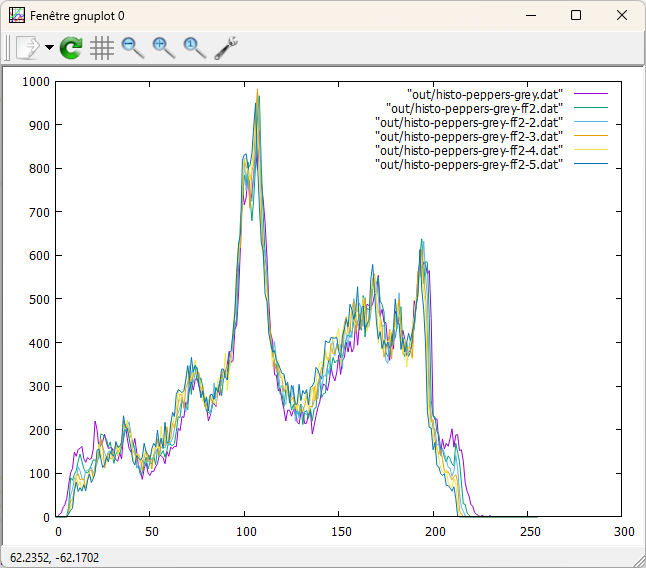
\includegraphics[width=.7\linewidth]{./out/histo-peppers-grey-ff2}}
        \caption{Histogramme de l'image floutée}\label{Fig:histo-peppers-grey-ff2}
    \end{figure}

    Comme pour le profil de ligne, on peut clairement voir ici que plus on floute l'image, plus l'histogramme devient
    lisse.

    \newpage
    \section{Floutage de l'image couleur}\label{sec:5}

    \subsection{Programme}\label{subsec:5.1}

    On commence par créer le programme \texttt{filtre\_flou\_couleur.cpp}.
    L'essentiel du code est le suivant :
    % insert code as image
    \begin{figure}[!htb]
        \centering
        \fbox{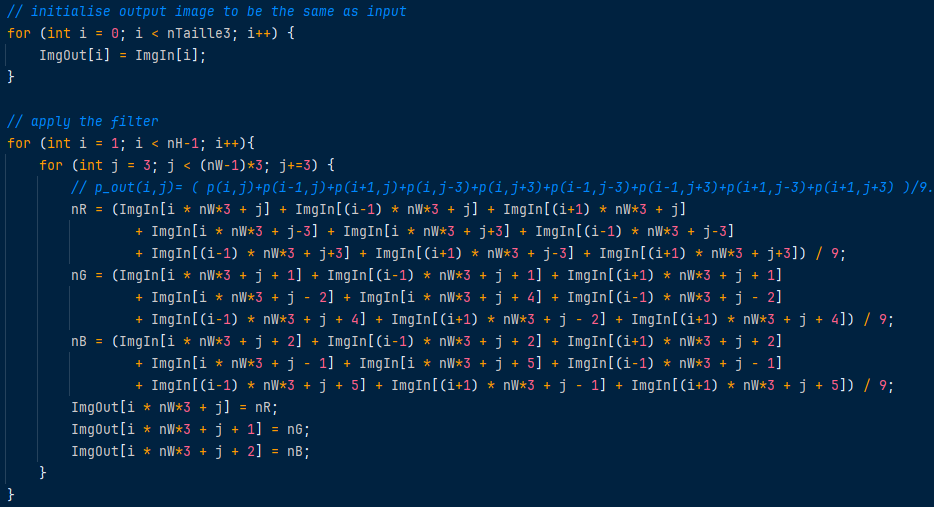
\includegraphics[width=.7\linewidth]{./out/code-filtre-flou-couleur}}
        \caption{Code du programme \texttt{filtre\_flou\_couleur.cpp}}\label{Fig:code-filtre-flou-couleur}
    \end{figure}

    On peut alors appliquer le programme à l'image \texttt{peppers.ppm}.
    Cela donne :
    % insert image and modified image side by side
    \begin{figure}[!htb]
        \begin{minipage}{0.48\textwidth}
            \centering
            \fbox{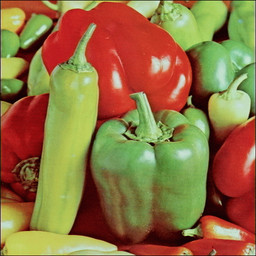
\includegraphics[width=.7\linewidth]{./out/orig-peppers}}
            \caption{Image originale}\label{Fig:peppers-1}
        \end{minipage}\hfill
        \begin{minipage}{0.48\textwidth}
            \centering
            \fbox{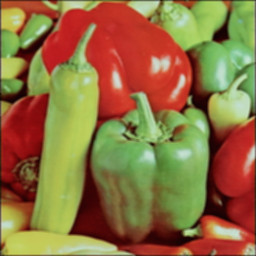
\includegraphics[width=.7\linewidth]{./out/peppers-ffc}}
            \caption{Image floutée}\label{Fig:peppers-ff}
        \end{minipage}
    \end{figure}

    \subsection{Comparaison des histogrammes}\label{subsec:5.2}

    On compare ensuite les histogrammes de l'image originale et de l'image floutée.
    Cela donne :
    % insert graph of histograms
    \begin{figure}[!htb]
        \centering
        \fbox{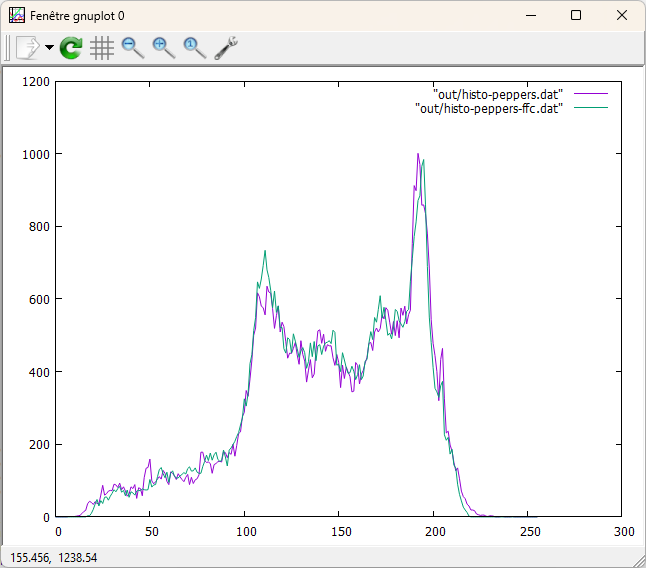
\includegraphics[width=.7\linewidth]{./out/histo-peppers-ffc}}
        \caption{Histogramme de l'image floutée}\label{Fig:histo-peppers-ffc}
    \end{figure}


\end{document}